\documentclass[aspectratio=43,english]{beamer}

\usepackage[english]{babel}

\usepackage[T1]{fontenc}
\usepackage[utf8]{inputenc}
\usepackage{lmodern}
\usepackage{pgfplots}
\usepackage{xifthen}
\usepackage{newunicodechar}
\usepackage{textcomp}
\usepackage[absolute,overlay]{textpos}
\usepackage{xparse}

\newunicodechar{°}{\textdegree}
\newunicodechar{µ}{\textmu}

\newcommand*{\ft}{\frametitle{\secname}}
\newcommand*{\ftsub}[1]{\frametitle{\secname\ - #1}}
\newcommand*{\itemp}{\item}
%\newcommand*{\itemp}{\pause\item}
\newcommand*{\+}{\texttt{+}}

\newcommand{\sectionframeimpl}[2]{
	\begin{frame}
	#1
	\begin{itemize}
	#2
	\end{itemize}
	\end{frame}
}
\NewDocumentCommand{\sectionframe}{s m m}{
	\IfBooleanTF{#1} {
		\section*{#2}
	} {
		\section{#2}
	}
	\sectionframeimpl{\ft}{#3}
}
\NewDocumentCommand{\subsectionframe}{s m m}{
	\IfBooleanTF{#1}{
		\subsection*{#2}
	} {
		\subsection{#2}
	}
	\sectionframeimpl{\ftsub{#2}}{#3}
}
\NewDocumentCommand{\subsubsectionframe}{s m m}{
	\IfBooleanTF{#1}{
		\subsubsection*{#2}
	} {
		\subsubsection{#2}
	}
	\sectionframeimpl{\ftsub{#2}}{#3}
}

\beamertemplatenavigationsymbolsempty

\mode<presentation>{
	\usetheme{Madrid}
	\usecolortheme{spruce}
}

\begin{document}

% "I want to give a overview about the Nouveau project and what challenges we deal with reverse engineering Nvidia GPUs. This includes security mechanisms Nvidia added over time to their GPUs to prevent us from doing our job. Having an open source GPU driver is important, because nearly everything somebody does on their Linux driven machine goes through the graphical stack and therefore a lot of sensible information goes through it and why should we trust closed source software with our stuff? Main topics will be which parts of the graphics stack we work on, our goals, what we have achieved already, what tools we are working with to trace the Nvidia driver, how somebody interested in this project can help out, what we currently are working on and what I would like to see implemented next."

% Topics:
% graphic stack parts
% goals
% tools
% current work
% wish list

% TODO: abbreviations

\title[Nouveau]{Nouveau}
\subtitle{Reverse Engineering Nvidia GPUs}
\author{Karol Herbst}
\date{}

\begin{frame}
\titlepage
\end{frame}

\section*{Introduction}
\subsectionframe*{Myself}{
	\itemp Worked as a Java Backend/Middleware developer since 2010
	\itemp No experience with embedded hardware before
	\itemp Started working on Nouveau to fix bugs end of 2015
	\itemp Joined Red Hat Graphics team in November 2017
}

\subsectionframe*{Motivation}{
	\itemp Getting more people interested
	\itemp Demystify what we do
	\itemp Getting others to use the same tools
}

\section*{Overview}

\begin{frame}
	\ft
	\setcounter{tocdepth}{1}
	\tableofcontents
\end{frame}

\sectionframe{Goals}{
	\itemp Understanding the hardware
	\itemp Completely open alternative to closed driver
	\itemp Being able to do research by tweaking
	\itemp To have fun!
}

\section{Facts}
\subsectionframe{General}{
	\itemp MIT licensed
	\itemp Started in 2005
	\itemp Accepted 2010 in Linux 2.6.33 as experimental
	\itemp Marked Stable in Linux 3.4
	\itemp Some BSD ports
	\itemp Supports most Nvidia GPUs (Riva TNT up to Geforce 10 series and Tegra SOCs)
}

\subsectionframe{Features}{
	\itemp OpenGL 4.3 (unofficial: 4.5)
	\itemp OpenGL ES 3.1
	\itemp D3D9 (Gallium Nine \+ wine)
	\itemp Video acceleration (XvMC, VDPAU)
	\itemp Hwmon - Linux HW Monitoring
	\itemp Various Power Management features
	\itemp[!] not all features supported on all GPUs
	\itemp[=>] it is not a toy project!
}

\section{Reverse Engineering}
\subsectionframe{Instruction Set Architectures}{
	\itemp Shader/CUDA cores
	\itemp fµc
	\itemp Tools: envydis, nvdisasm
	\pause\only<2>{
		\begin{textblock*}{5cm}(0.1cm,3.4cm)
			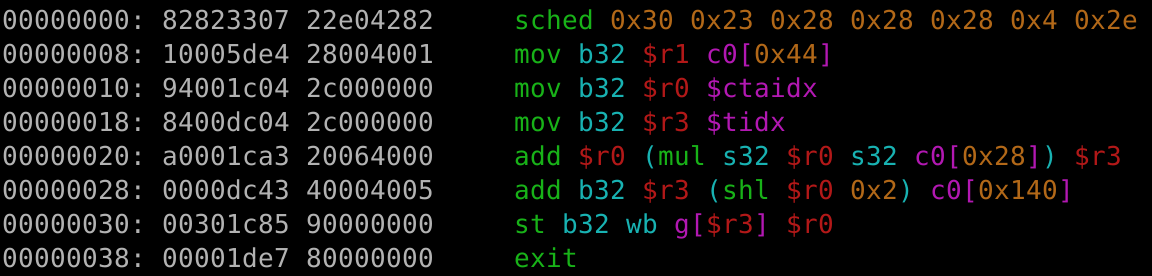
\includegraphics[scale=0.413]{envydis}
		\end{textblock*}
	}
}

\subsectionframe{GPIO and I²C devices}{
	\itemp Sensors
	\itemp Fans
	\itemp Voltage control
	\itemp LEDs
}

\subsectionframe{Memory Mapped I/O}{
	\itemp Many "registers"
	\itemp Engines
	\begin{itemize}
		\itemp PDISP (Display Engine)
		\itemp PGRAPH (Rendering Engine)
		\itemp Video Engines
		\itemp PMU
		\itemp many more
	\end{itemize}
	\itemp Tools: mmiotrace \+ demmio, envydis
}

\subsubsectionframe{Mmiotrace}{
	\itemp In-kernel tracer for MMIO
	\itemp Traces communication between a kernel driver and its devices
	\itemp "abuses" Page faults:
	\begin{enumerate}	
		\itemp Marks mapped pages as non existing
		\itemp Page faults on memory access
		\itemp Parses and single steps next instruction
		\itemp continue
	\end{enumerate}
	\itemp demmio (enytools) used to parse traces
	\pause\only<2>{
		\begin{textblock*}{5cm}(0.1cm,2.4cm)
			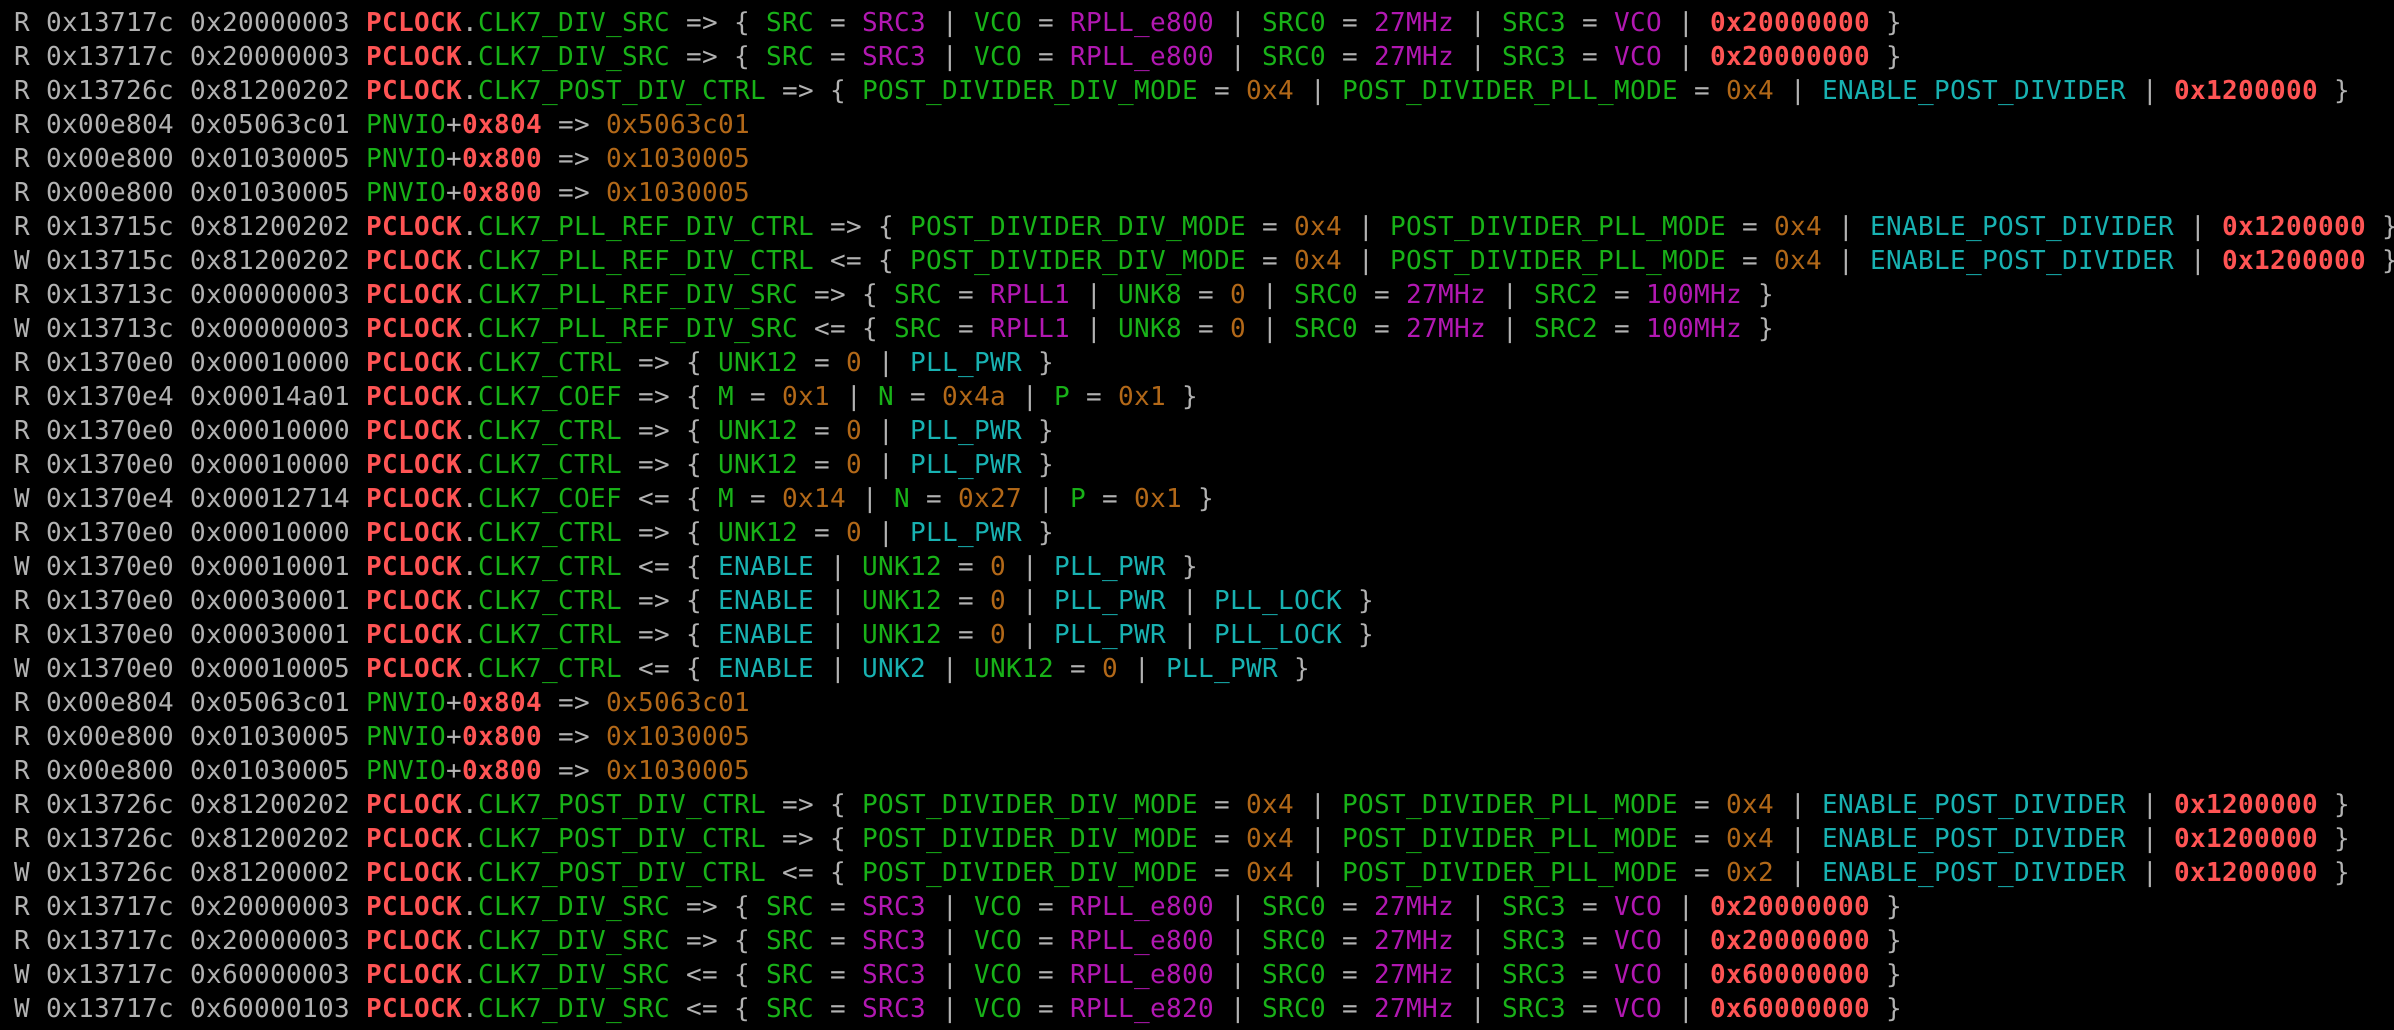
\includegraphics[scale=0.199]{mmiotrace_reclocking}
		\end{textblock*}
	}
}

\subsectionframe{VBIOS}{
	\itemp Describes the GPU
	\itemp Meaning of Tables
	\itemp Changing values and monitoring for runtime changes
	\itemp Guessing
	\itemp Can be automated
	\itemp Tool: nvbios
}

\subsectionframe{Software}{
	\itemp Nvidias
	\begin{itemize}
		\itemp OpenGL/Vulkan (for Graphics)
		\itemp VDPAU (Linux API for video acceleration)
		\itemp OpenCL/CUDA (for Compute)
	\end{itemize}
	\itemp[] Implementation
	\itemp various Command Line Tools
	\itemp Tools: valgrind-mmt, demmt
}

\section{Development}
\subsectionframe{Kernel driver}{
	\itemp Object-Oriented C Code
	\itemp Implements DRM APIs (Direct Rendering Manager)
	\begin{itemize}
		\itemp Display (via KMS - kernel modesetting)
		\itemp Access from Userspace
		\itemp Memory Management (TTM)
		\itemp Rendering
	\end{itemize}
	\itemp Hwmon
	\itemp Power Management
}

\subsectionframe{X11 Server Driver / 2D acceleration}{
	\itemp packages: xf86-video-nouveau
	\itemp native 2D hardware acceleration
	\itemp OpenGL can be used instead as well (via xf86-video-modesetting)
}	

\subsectionframe{Mesa / 3D acceleration}{
	\itemp OpenGL (ES)
	\begin{itemize}
		\itemp Implementation of Gallium API
		\itemp Implementation of new OpenGL(ES) Extensions
		\itemp codegen (Shader Compiler)
		\begin{itemize}
			\itemp SSA based backend compiler
			\itemp optimisation passes
		\end{itemize}
	\end{itemize}
	\itemp VDPAU
	\itemp OpenCL (WIP)
	\itemp Vulkan (TODO)
}

\subsectionframe{OpenGL}{
	\itemp Driver/Backend
	\itemp API
	\itemp Extensions
	\itemp Khronos Conformance Test Suite
}

\sectionframe{Working with Nvidia}{
	\itemp Provides basic Documentation for basic features
	\itemp Open-Source Android Driver (will be replaced by Nouveau?)
	\itemp Signed firmware for Maxwell2\+
}

\sectionframe{Current Challenges}{
	\itemp Pass Khronos CTS for exposing OpenGL 4.4\+
	\itemp Improving Performance
	\itemp build a CI system (ezbench maybe?)
	\itemp Maxwell2\+
	\begin{itemize}
		\itemp Signed VBIOS
		\itemp Signed Firmware
		\begin{itemize}
			\itemp Fan control
			\itemp Reclocking (since Pascal)
		\end{itemize}
		\itemp Harder REing of VBIOS and MMIO registers
	\end{itemize}
	\itemp Compute support (OpenCL, Vulkan Compute)
}

\sectionframe{How to help}{
	\itemp Own hardware with bugs running Nouveau and fix those
	\itemp Be interested and motivated
	\itemp GSoC/EVoC (for students)
}

\sectionframe*{Links}{
	\item IRC Channel on freenode: \href{ircs://chat.freenode.net:6697/\#nouveau}{\#nouveau}
	\item Mailing list: \url{https://lists.freedesktop.org/mailman/listinfo/nouveau}
	\item Trello Board: \url{https://trello.com/b/ZudRDiTL/nouveau}
	\item GSoC/EVoC project ideas: \url{https://www.x.org/wiki/SummerOfCodeIdeas/}
}

\end{document}